\documentclass[12pt]{article}
\usepackage[margin=1.0in]{geometry}
\usepackage{hyperref}
\usepackage{amsmath}
%\usepackage{amsmath}
\usepackage{graphicx}
% \usepackage[extendedchars]{grffile}
\usepackage{chngpage}
\usepackage{calc}


\title{Propagation of simulated millicharged particles to the Milliqan detector}

\author{C. Campagnari, B. Marsh (UCSB), F. Golf (UNL)}

\setlength{\parindent}{0em}
\setlength{\parskip}{1em}

\begin{document}
\maketitle


\section{Introduction}
In this note we describe the procedure used to propagate simulated millicharged
particles (mCPs) through the CMS environment to the Milliqan detector face. The goals 
of this are to (1) calculate the acceptance of the Milliqan detector (and thus,
when combined with $\sigma\times\mathcal{B}$, the rate of incidence of mCPs),
and (2) generate ``hits'' on the Milliqan detector face  (position and momentum of incoming mCPs)
that can be fed into more sophisticated Geant4 simlations of the detector.

There are four main components to this simulation, listed here and then described in more
detail in the following sections:
\begin{enumerate}
\item Propagation through the CMS magnetic field
\item Multiple scattering while traveling through matter
\item Energy loss while propagating through matter
\item Computation of intersection with Milliqan detector face
\end{enumerate}

All of the code for the propagation is contained in the \href{https://github.com/bjmarsh/MilliqanSim}{\underline{\bf MilliqanSim}} GitHub repository.

\section{Propagation through the CMS magnetic field}
At its core the simulation uses a fourth-order Runge-Kutta integrator to step a charged particle
through a magnetic field. The basic equations of motion are
\begin{equation}\label{eq:dxdt}
\frac{d\vec{x}}{dt} = \vec{v} = \frac{\vec{p}c^2}{E} = \frac{\vec{p}c^2}{\sqrt{(\vec{p}c)^2+(mc^2)^2}},
\end{equation}
\[
\frac{d(\vec{p}c)}{dt} = qc\;\vec{v}\times\vec{B}.
\]
If $B$ is in Tesla, $t$ in ns, velocity in m/ns, charge in units of $e$, and $\vec{p}c$ in MeV, the latter becomes
\begin{equation}\label{eq:dpdt}
\frac{d(\vec{p}c)}{dt} = 89.8755\;q\;\vec{v}\times\vec{B}.
\end{equation}

\begin{figure}
\centering
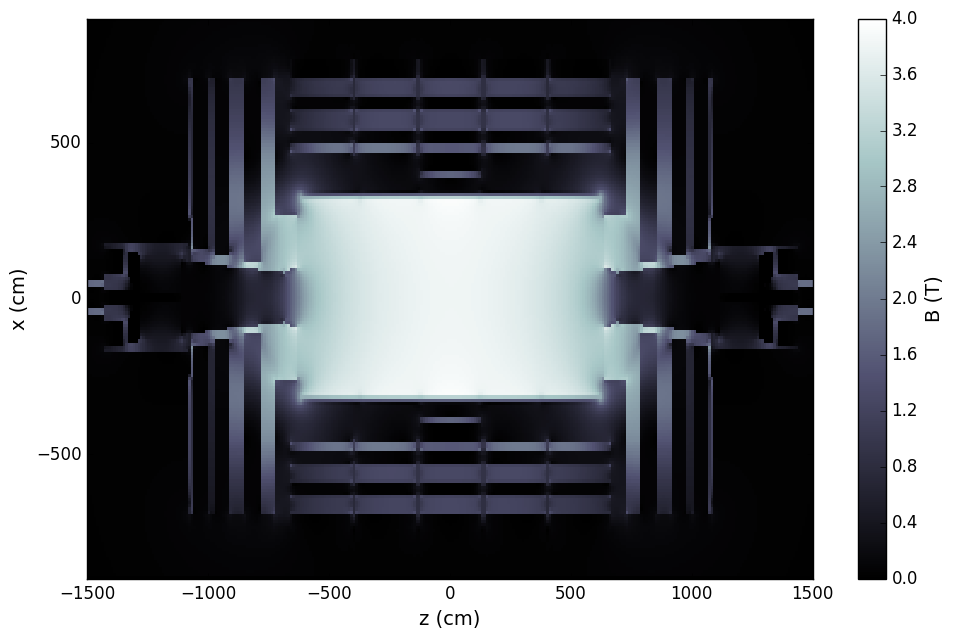
\includegraphics[width=0.7\textwidth]{plots/cms_bfield_coarse.png}
\caption{Magnitdue of the CMS magnetic field, in the $y=0$ plane.}
\label{fig:bfield}
\end{figure}

The magnetic field for CMS has been extracted from CMSSW
in a 3-dimensional cylindrical grid in increments of $\Delta r=10$ cm, $\Delta z=10$ cm, $\Delta\theta=5^\circ$, out to
$r=10$ m and $z=\pm15$ m. A map of the magnitude in the $y=0$ plane is shown in Fig.~\ref{fig:bfield}.
[\emph{Note: we extracted this B-field map from CMSSW, which isn't public. But there are CMS publications (\href{https://iopscience.iop.org/article/10.1088/1748-0221/5/03/T03021/meta}{example}) that measure
this, so I guess we can plausibly say we got it from those.}]

At each timestep, the magnetic field is determined from ths pre-loaded map and used in the equation of motion (\ref{eq:dpdt}).
The field is interpolated between the two nearest points in $r$ (not $z$ or $\theta$, since for the region of interest the field
is essentially flat over these variables).

For now, the simulation uses a timestep of $dt=0.1$ ns, corresponding to a distance $dx\approx3$ cm for a particle traveling near
the speed of light. This can probably be increased without meaningfully changing the results, in order to speed up computation time.


\section{Multiple scattering through matter}
In order to simulate the interactions of particles with matter, a very simple schematic of CMS and the surrounding environment has been defined:
\begin{itemize}
\item $1.29 \leq r < 1.8$ m: PbWO$_4$ (ECAL)
\item $1.8 \leq r < 7$ m: iron (HCAL, magnet, iron return yokes)
\item $16\leq R\leq33$ m: ``standard rock'' (as defined by PDG \cite{PDG_properties})
\item everything else: ``air'' (as defined by PDG \cite{PDG_properties})
\end{itemize}

The implementation of multiple scattering is taken from the PDG chapter on the passage of particles through matter \cite{PDG_matter}.
This assumes a small-angle gaussian scattering, and does not take into account non-gaussian tails from rare hard scatters. However,
we are interested only in the ``bulk'' of the distribution, so this approximation should be fine.

The RMS of the scattering angle distribution is given by
\begin{equation}\label{eq:thrms}
\theta_0 = \frac{13.6~\text{MeV}}{\beta cp}\;z\;\sqrt{\frac{x}{X_0}}\left[1 + 0.088\log_{10}\left(\frac{xz^2}{X_0\beta^2}\right) \right],
\end{equation}
where $p$, $\beta c$, and $z$ are the momentum, velocity, and charge number of the incident particle, $x$ is the distance traversed, and 
$X_0$ is the radiation length of the material.

In addition to an angular deflection $\theta_\text{plane}$, there is a correlated transverse deviation $y_\text{plane}$ (see Fig. \ref{fig:mscangles}). The correlation coefficent
turns out to be $\sqrt{3}/2\approx0.87$, and it is sufficient to generate two independent gaussian random variables $z_1,z_2$ and compute
\begin{equation}\label{eq:msc}
y_\text{plane} = z_1\;x\;\theta_0/\sqrt{12} + z_2\;x\;\theta_0/2
\end{equation}
\[
\theta_\text{plane} = z_2\;\theta_0.
\]

This is done independently in both directions orthogonal to the direction of travel.

\begin{figure}
\centering
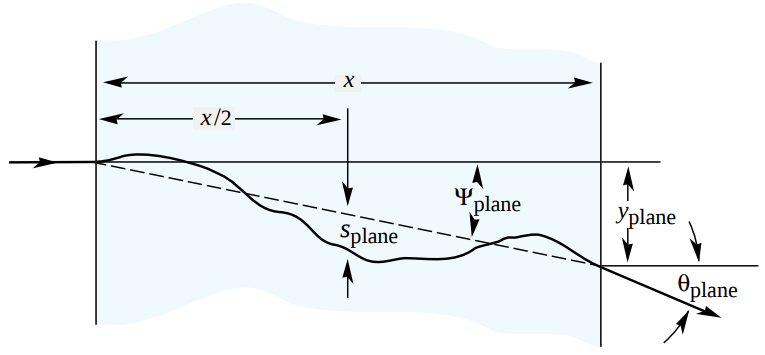
\includegraphics[width=0.7\textwidth]{plots/pdg_msc_diagram.png}
\caption{Diagram showing the defined $\theta_\text{plane}$ and $y_\text{plane}$ variables used to describe multiple scattering.}
\label{fig:mscangles}
\end{figure}

\section{Energy loss}
In addition to multiple scattering, particles lose energy as the propagate through matter. This is implemented using the 
Bethe formula
\begin{equation}\label{eq:dedx}
\left\langle-\frac{dE}{dx}\right\rangle = Kz^2\frac{Z}{A}\frac{1}{\beta^2}\left[\frac{1}{2}\log\frac{2m_ec^2\beta^2\gamma^2W_\text{max}}{I^2} - \beta^2 - \frac{\delta(\beta\gamma)}{2} \right].
\end{equation}

For definitions of all terms and parameters, see \cite{PDG_matter}. All material constants are taken from \cite{PDG_properties}.

\section{Putting it all together}
At each timestep, the following steps are taken:
\begin{enumerate}
\item Evaluate $d\vec{x}/dt$ and $d\vec{p}/dt$ using using the current position/momentum $\vec{x}_x/\vec{p}_i$ inserted into Eqs. \ref{eq:dxdt} and \ref{eq:dpdt} (actually,
evaluate four times as per the Runge-Kutta method). Use the Runge-Kutta method to compute $\Delta\vec{x}_{\text{B},i}$ and $\Delta\vec{p}_{\text{B},i}$ for the timestep.
\item Look up the material at $\vec{x}_i$, and plug the material constants into Eq. \ref{eq:thrms}. Then use Eq. \ref{eq:msc} to compute a transverse displacement
and angular deflection (independently for both transverse directions). Combine to get $\Delta\vec{x}_{\text{MS},i}$ and $\Delta\vec{p}_{\text{MS},i}$ due to multiple scattering.
\item Use material constants to evaluate $dE/dx$ with Eq. \ref{eq:dedx}. Multiply by $\delta x=v\delta t$ to get $\delta E$, and use this to compute $\Delta\vec{p}_{\text{EL},i}$.
\item The total changes in position and momentum for the timestep are then $\Delta\vec{x}_i = \Delta\vec{x}_{\text{B},i}+\Delta\vec{x}_{\text{MS},i}$ and
$\Delta\vec{p}_i = \Delta\vec{p}_{\text{B},i}+\Delta\vec{p}_{\text{MS},i}+\Delta\vec{p}_{\text{EL},i}$.
\end{enumerate}

This is done for $N_\text{steps}$ timesteps (or until a specified distance cutoff is reached). At the end we get an array of $(t,x,y,z,p_x,p_y,p_z)$ values at each timestep.

\section{Intersection with the Milliqan Detector}
To facilitate acceptance and rate calculations, tools have been added to the simulation to compute intersections with
various detector models.

For simple applications, one can find intersections with an external plane and retrieve the position and momentum
at the intersection. This is useful for gathering four-vectors to feed into an external simulation of the detector.

The ability to construct a ``Milliqan-type'' detector with arbitrary numbers of bars has also been added.
The entry/exit points for each individual bar can be computed, so that for each trajectory one can determine
the number of bars hit, whether those bars are in a line, the length of the path traversed within the bar, etc.
An example of two mCPs hitting the Milliqan demonstrator is shown in Fig. \ref{fig:traj_vis}.

\begin{figure}
\centering
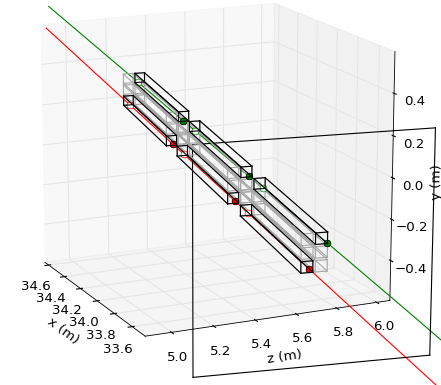
\includegraphics[width=0.7\textwidth]{plots/traj_vis.png}
\caption{Visualization of two mCP trajectories passing through the Milliqan demonstrator.}
\label{fig:traj_vis}
\end{figure}


\begin{thebibliography}{1}

\bibitem{PDG_properties}  PDG, ``Atomic and Nuclear Properties of Materials''.
[\href{http://pdg.lbl.gov/2019/AtomicNuclearProperties/index.html}{link}]

\bibitem{PDG_matter}  PDG, chapter 33. ``Passage of particles through matter''.
[\href{http://pdg.lbl.gov/2019/reviews/rpp2018-rev-passage-particles-matter.pdf}{link}]
  
\end{thebibliography}
  
\end{document}
